\documentclass[12pt,letterpaper]{article}

\usepackage{amsmath, amsthm, amssymb, amsfonts}
\usepackage{graphicx}
\usepackage{bm}
\usepackage{natbib}

\theoremstyle{definition}
\newtheorem{dfn}{Definition}

\begin{document}

% The numbers below controls the amount of space between the following sections
\def\shiftdowna{0.32in}  % Adjust for balance
\def\shiftdownb{0.22in}  % Adjust for balance

% Set up the boiler plate at the top of the page

\begin{center}
\textbf{{\large Project Work Statement}}\\


% SPONSOR
\vspace \shiftdowna
\underline {Sponsor}\\ 
\vspace{5pt}
\textbf{{\large Washington Metropolitan Area Transit Authority}}\\
\vspace{5pt}
\textbf{{\large Maryland Transit Administration}}\\


% TITLE
\vspace \shiftdowna
\textbf{{\large Logistics of Constructing a Washington D.C.-Baltimore Rapid Transit Line}}


% STUDENTS
\vspace{0.35in}
\vspace \shiftdownb
\underline {Participants} \\
\vspace{5pt}
\text{Danni Tang}, \texttt{danni@jhu.edu}

% SPONSORS
\vspace \shiftdownb
\underline {Academic Mentor}\\
\vspace{5pt}
Nam H. Lee, \texttt{nhlee@jhu.edu} \\

% DATE
\vspace \shiftdowna
Date: \today

\end{center}

\vfill  
%Fill page to force following note to bottom
\footnoterule
\noindent \small{Any apparent association of this work to WMATA and MTA is
fictional one, and the sole purpose of this work is a class exercise.}

\newpage

\section{Background} 
The Washington Metropolitan Area Transit Authority (WMATA) is a transportation agency created by the Library of Congress to provide rapid transit between the District of Columbia, Maryland, and the Commonwealth of Virginia. WMATA provides rapid transit service (Metrorail), bus services (Metrobus), and paratransit (MetroAccess). The agency works to facilitate ongoing transportation, promote transportation planning and expand its current system to other regions of the three states. The Maryland Transit System (MTA Maryland) is a state-operated agency that provides mass transportation in the Baltimore-Washington Metropolitan area, serving as a major transit provider for a large population of Baltimore residents. MTA Maryland serves numerous bus lines, as well as the Light Rail, Metro Subway, and the MARC train. Together, the two transportation agencies provide separate but convenient fast transit in the Greater Washington-Baltimore Metropolitan area.

\section{Problem Statement}
Although the WMATA is currently constructing two new lines surrounding D.C. to the existing metro system, it has no plans to expand the Metrorail system to the city and suburbs surrounding Baltimore, as demonstrated by Figure \ref{fig:wmatamap}. MTA Maryland's Metro Subway system only operates within the city limits. Residents of the Greater Washington-Baltimore Metropolitan area therefore have limited access to public transportation between the two cities. Currently, the MARC and AMTRAK are the only two trains that travel directly between D.C. and Baltimore; however, the MARC only operates during weekday rush hours, and AMTRAK fares are too impractical for daily commute. 
The sponsors currently have no plans to build such a crucial transit line, as the two metro systems operate under two different government agencies. Our task is to provide them with a model that can demonstrate and predict the operating capacity for such a line if it were to be built by employing existing published Maryland transportation statistics, such as traffic volume and highway mobility reports between D.C. and Baltimore.
\begin{figure}[h]
    \begin{center}
        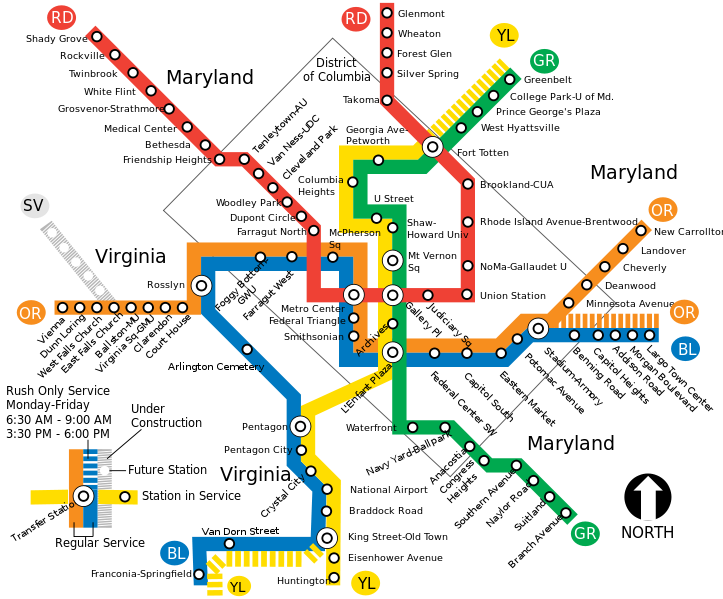
\includegraphics[width=\textwidth]{WMATA_system_map.png}
    \end{center}
    \caption{WMATA existing lines and stations, June 2012}
\end{figure}


\section{Approach}
We will gather data and statistics published by the Maryland Department of Transportation to incorporate them into a mathematical model of traffic flow. We will consider the Payne-Whitham or the Aw-Rascle equations for traffic flow, which are second order equations that do not model individual vehicles, but rather the continuous vehicle density function and the continuous velocity function. We may also consider another model, proposed by M. Bando, which describes the optimal velocity in traffic, which takes into account Newtonian acceleration. Time permitting, we will also attempt to design an efficient subway line based on these models that can eliminate common factors such as traffic jam, vehicle density, time delays, and highway accidents. Based on resource allocation, time allowed, and the results of our research, we hope to develop a model that can provide fast, affordable transit that operates on a 24/7 basis for the residents of the Greater Washington-Baltimore Metropolitan area.
\section{Milestones}
We have the following major deadlines:
\begin{itemize}
    \item Work Statement due date, Sep 28, 2012,
    \item Midterm Presentation due date, Oct 12, 2012,
    \item Progress Report due date, Oct 26, 2012,
    \item Final Presentation due date, Nov 6, 2012,
    \item Final Report due date, Nov 30, 2012.
\end{itemize}

\section{Deliverable}
\subsection{From Team to Sponsor} % (fold)
The following outputs are expected from this project:
\begin{itemize}
    \item Mathematical model of the dynamic traffic flow at various hours of the day (morning, noon, and evening) on highways I-495 and I-95
    \item Analytical report on the results of traffic flow model to determine if a subway line is viable
    \item Time permitting, design of the aforementioned subway line, including fares, stops, and operating capacity
    \item R package with a complete set of documentations along with some test 
        codes that can be used to reproduce our numerical and simulation test
        results,
    \item Technical report and presentations summarizing the work. 
\end{itemize}

\subsection{From Sponsor to Team} % (fold)

In order for our project to be of successful one, we will need:
\begin{itemize}
    \item The most recent data and stastistics from the Department of Transportation by Oct 19, 2012. If circumstances change and we do not receive the required data, we will obtain traffic data made available for the public from past years from the Maryland Department of Transportation website.
    \item Computing resources, such as programming and modeling software
    \item Timely responses to inquiries, 
    \item Small expenses relevant to work.
\end{itemize}

Blablabla said Nobody ~\cite{Nobody06}.

\bibliographystyle{plain}
%%\renewcommand\bibname{Selected Bibliography Including Cited Works}
%\nocite{*}
\bibliography{mybib}{}
\end{document}
